\subsection{Rotationsgeschwindigkeitsabhängigkeit von Schichtdicken\label{sec:rotgeschw}}
Gemäß der Anleitung~\cite{Anleitung} folgt die Schichtdicke einer gespincoateten Polymerporbe der Schubert-Gleichung:

\begin{equation}\label{eq:schubert}
    d = A \cdot \left(\frac{\SI{1950}{\per\minute}}{\omega}\right)^\frac{1}{2} \cdot \left(\frac{c_0}{\SI{20}{\gram\per\litre}}\right) \cdot \left(\frac{M_W}{\SI{100}{\kilo\gram\per\mol}}\right)^\frac{1}{4}
\end{equation}
mit der Rotationsgeschwindigkeit $\omega$, der Konzentration $c_0$ und dem Molekulargewicht $M_W$ des Polymers. $A$ ist ein Skalierungsfaktor.

Nun werden die Schichtdicken $d$ der Proben mit konstanter Ausgangskonzentration 
\begin{equation*}
    c_0 = \SI{100}{\milli\gram\per\milli\litre}
\end{equation*} 
für die Transmissions- und Reflektionsmessungen in Abhängigkeit der Rotationsgeschwindigkeit $\omega$ des Spincoaters in Abb.~\ref{fig:schubertfit} dargestellt.

\begin{figure}[h!]
    \centering
    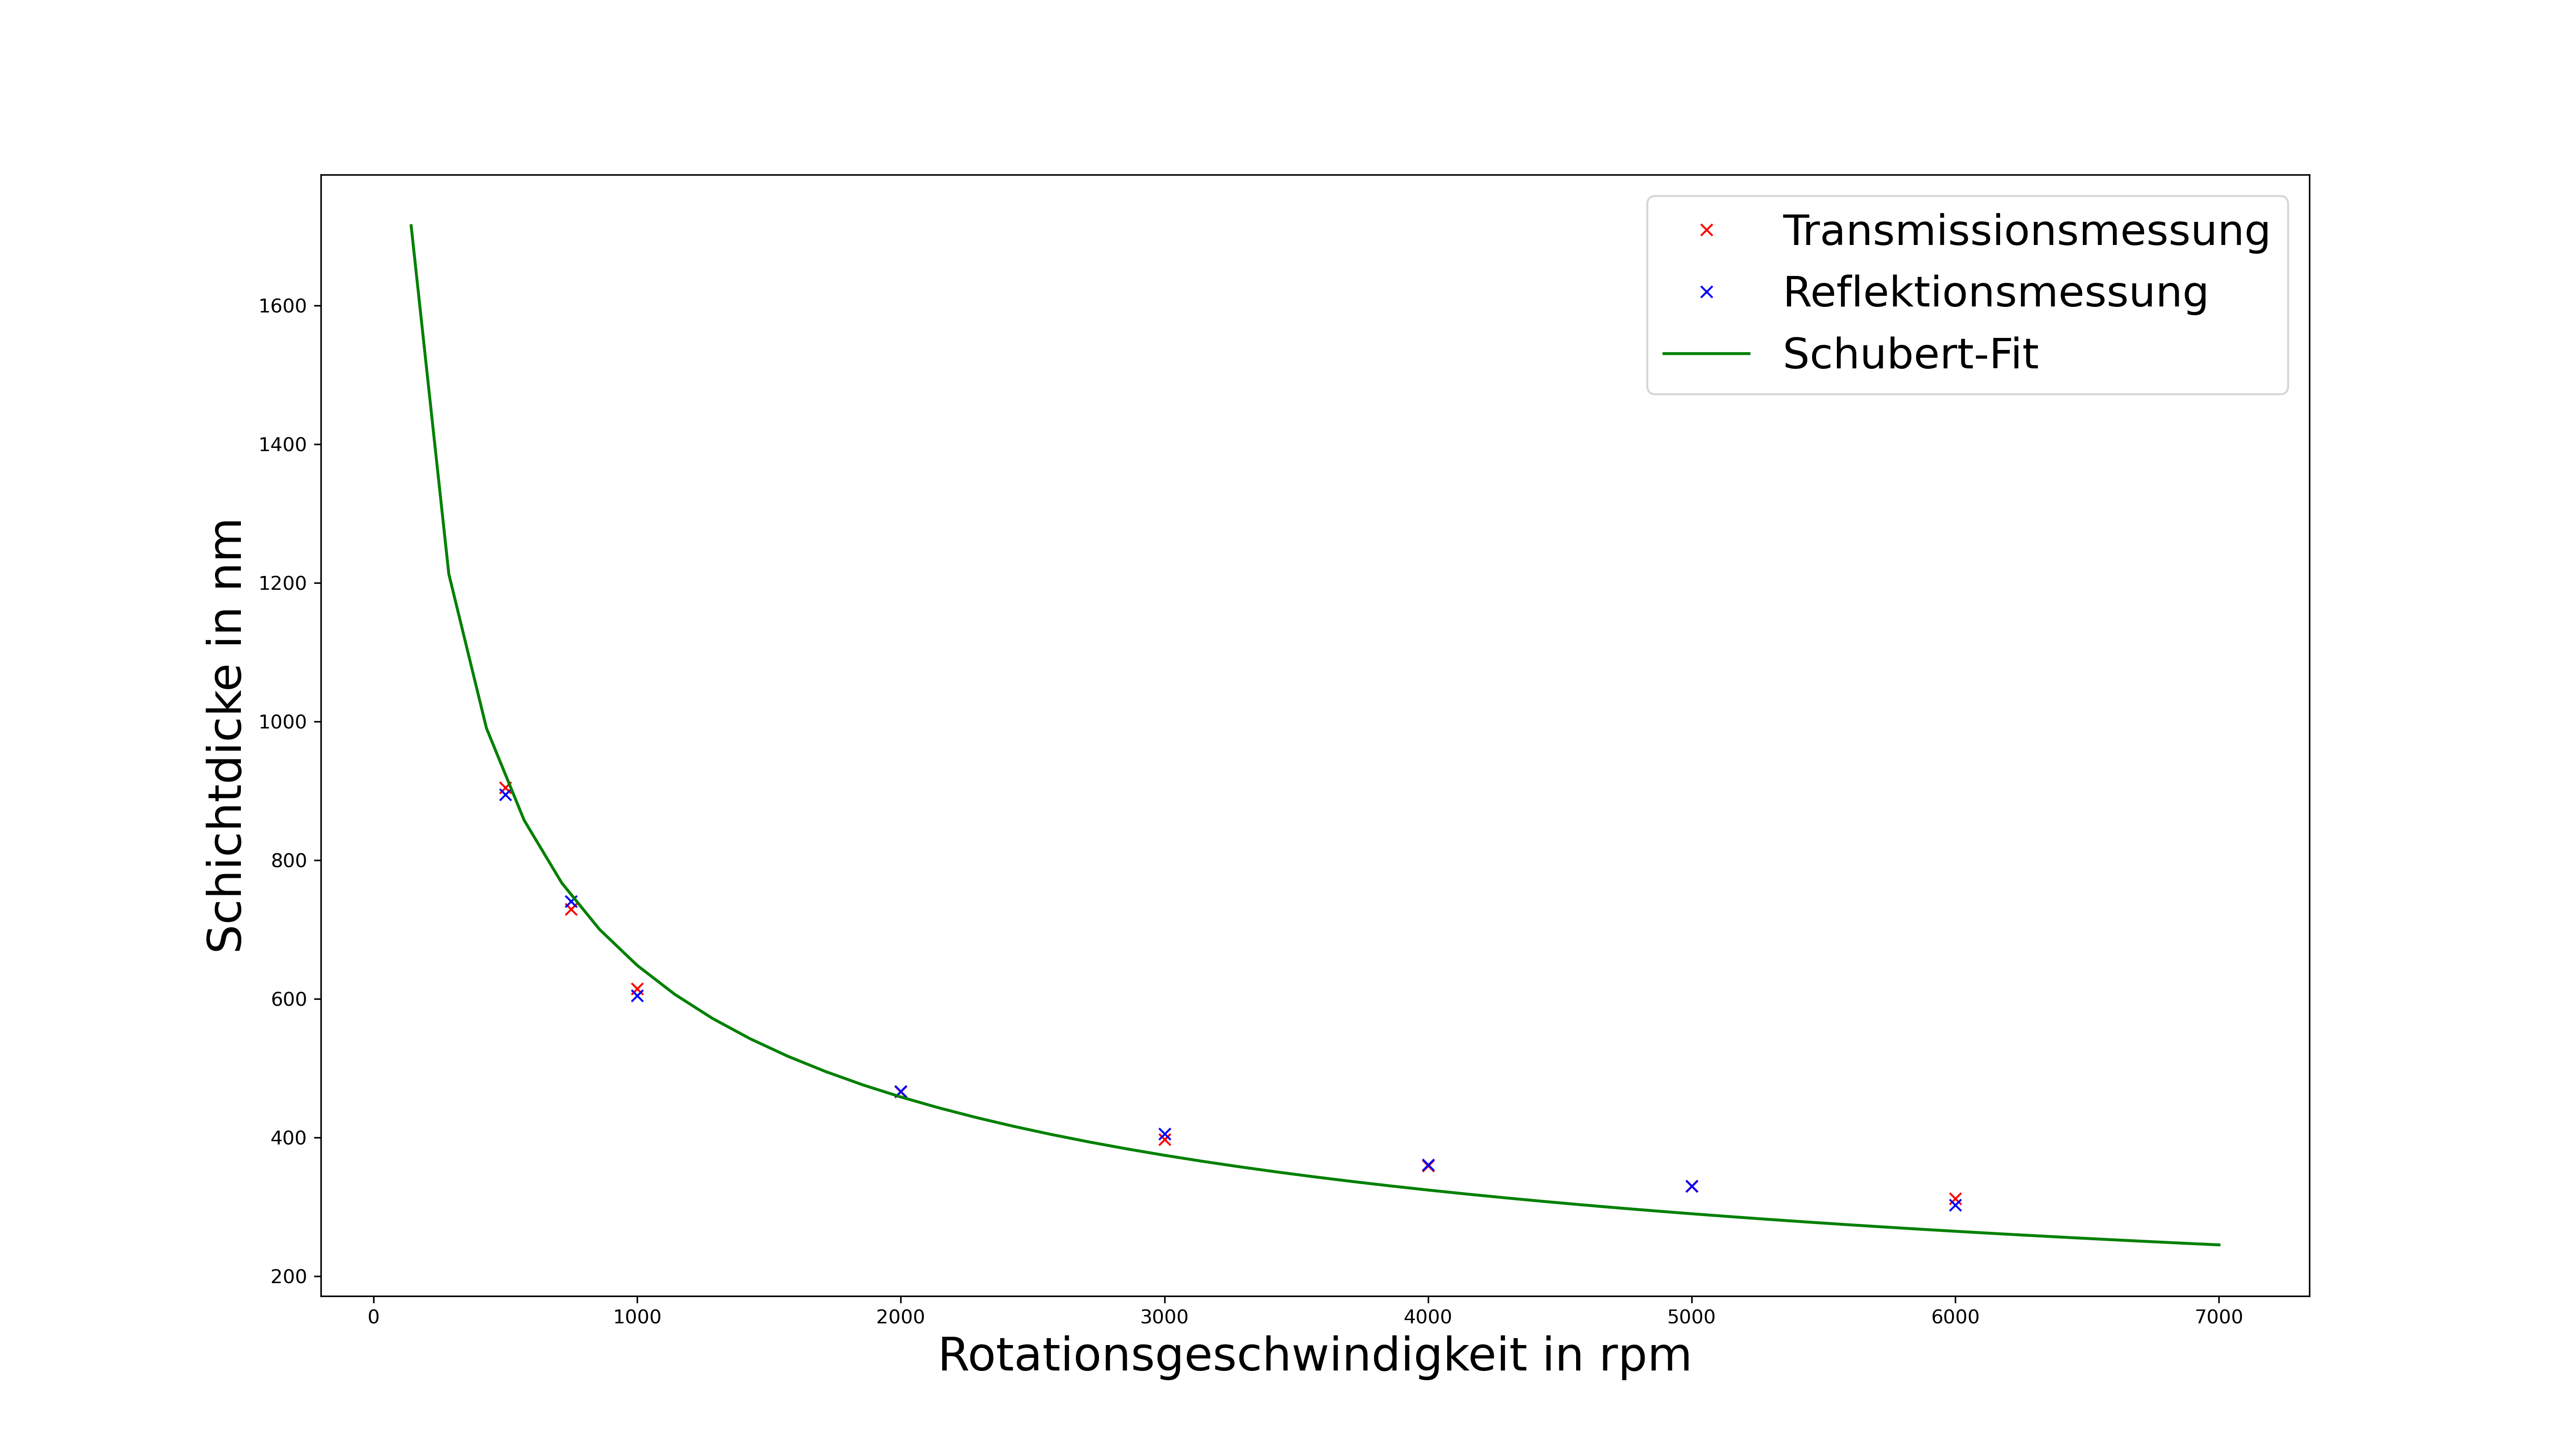
\includegraphics[width=0.8\linewidth]{schubertfit.png}
    \caption{Reflektions- und Transmissionsmessungen der Schichtdicken in Abhängigkeit der Rotationsgeschwindigkeit des Spincoaters mit zusätzlichem Fit nach der Schubert-Gleichung. Dargestellt ist nur der Fit für die Transmissionsmessungen, da der Reflektionsfit ununterscheidbar ähnlich ist.}
    \label{fig:schubertfit}
\end{figure}

Der Fitparameter $A$ beträgt
\begin{equation*}
    A = \SI{120,7(2,5)}{\metre}
\end{equation*}

Es fällt auf, dass der Fit insgesamt gut passt, besonders aber zu niedrigen Rotationsgeschwindigkeiten bzw.~höherer Schichtdicke, das Wurzelverhalten des Fits $d \propto \frac{1}{\sqrt{\omega}}$ ist gut erkennbar. Im Fit ist der x-Achsen Bereich bereits etwas höher gefasst als der tatsächliche Bereich der Rotationsgeschwindigkeiten, bei weiterer Extrapolierung der Messwerte geht die Schichtdicke für hohe Rotationsgeschwindigkeiten gegen 0 und für kleine Geschwindigkeiten wird die Schichtdicke schnell sehr hoch. Eine Geschwindigkeit von 0 rpm entspricht dem Fall des Auftragens der Lösung auf ein sich gar nicht rotierendes Substrat. Dabei könnten sich sehr leicht einzelne Tropfen bilden, was einer Verschlechterung der Filmhomogenität entspricht. 